\documentclass[a4paper,12pt]{article}
\usepackage{amsmath}
\usepackage{enumerate}
\usepackage{graphicx}

\pagestyle{empty} \setlength{\parindent}{0mm}
\addtolength{\topmargin}{-0.5in} \setlength{\textheight}{9in}
\addtolength{\textwidth}{1in} \addtolength{\oddsidemargin}{-0.5in}


\begin{document}
\title{Final Homework}
\author{Matt Forbes}
\date{December 7, 2010}
\maketitle

\section*{Problem 1}

\begin{enumerate}[]
  
\item The cost of going from exit $j$ to $k$ is $C_j + C_{j+1} +
  C_{j+2} + \dots + C_{k-1}$. I propose the data structure $H$ such
  that $H_i = C_1 + C_2 + \dots + C_{i-1}$. To calculate the cost exit
  $j$ to $k$ using $H$, it would simply be $H_k - H_j$. This
  expression expands to $(C_1 + C_2 + \dots + C_{j-1}) - (C_1 + C_2 +
  \dots + C_{k-1})$, which simplifies to $C_j + C_{j+1} + \dots +
  C_{k-1}$. Showing that $H_k - H_j$ is equivalent to the cost we
  calculated for exit $j$ to $k$. Given that $H$ is already
  calculated, this computation is a simple subtraction, $O(1)$.

\item Generating this data structure is very easy and would take
  $O(n)$ time and holds $n$ elements. Each element $H_i$ is equal to
  $C_i + H_{i-1}$ which lends itself easily to an accumlating loop
  from $1$ to $n$.

\item
\begin{verbatim}
H[1] = C[1]
for i = 2...n:
  H[i] = C[i] + H[i-1]
\end{verbatim}
  
\end{enumerate}

\section*{Problem 2}

\begin{center}
  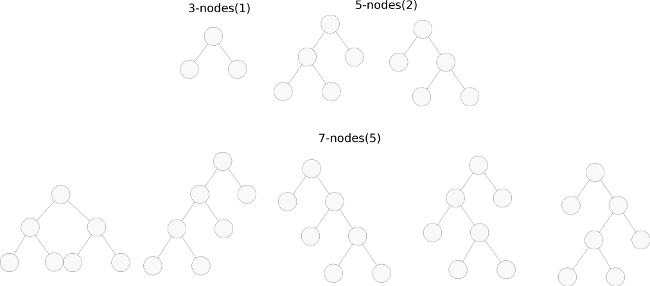
\includegraphics[width=450px, height=225px, keepaspectratio=true]{image/fulltrees.png}
\end{center}

\begin{enumerate}[a)]

\item $B_3 = 1, B_5 = 2, B_7 = 5$.

\item You can't construct a full binary tree with an even number of
  nodes. Every node always has zero or two child nodes, meaning
  everytime the tree grows, it must grow by a multiple of two
  nodes. So starting with the root, and growing $n$ times, the total
  number of nodes will always be of the form $1 + 2n$, which is odd.

\item \[B_n = \left\{
      \begin{tabular}{l r}
        1 & $n=1, n=3$\\
        apples & $n > 3$
      \end{tabular}
      \right\}\]

\end{enumerate}


\end{document}
